\documentclass{soups}

\usepackage[backend=biber]{biblatex} %for bibliography
\addbibresource{Bibliography.bib} %specify location of .bib (bibtex) file
\usepackage{url} %for using urls in bibliography entries
\usepackage{graphicx} %for figures

\pdfpagewidth=8.5truein
\pdfpageheight=11truein

\usepackage{enumitem}

\usepackage{pdfpages}
\usepackage{url}
\usepackage{tikz}
\usetikzlibrary{shapes, arrows}
\usepackage{times}
\usepackage{balance}
\renewcommand{\topfraction}{0.99} % be more aggressive about text around floats
\renewcommand{\floatpagefraction}{0.99}
\pagestyle{plain} % page numbers


\title{Visualizing the Impact of Organizational Change}
\subtitle{Project proposal}

\numberofauthors{2}

\author{
\alignauthor
Rob Barwell\\ %\titlenote{Dr.~Trovato insisted his name be first.}\\
       \affaddr{Carleton University}\\
       \affaddr{Ottawa, Canada}\\
       \email{rob@barwell.ca}
% 2nd. author
\alignauthor
Eric Spero\\ %\titlenote{The secretary disavows any knowledge of this author's actions.}\\
       \affaddr{Carleton University}\\
       \affaddr{Ottawa, Canada }\\
       \email{eric.spero@carleton.ca}
}

\begin{document}

\nobalance

\makeatletter
\def\@copyrightspace{\relax}
\makeatother

\maketitle

\section{Description}

We plan to design and develop a novel visualization to support managerial decision-making by helping managers understand the effects of personnel change on an organization.

\section{Reading Review}

The rise of the \lq gig economy\rq{}\cite{de2015rise,friedman2014workers} has forced society through a massive transition in the past two decades with people transitioning between jobs with greater frequency.  Historically, a person would obtain a job from high school or university and stay with a specific company until they retire.  This resulted in organizations that had minimal change, which could be easily managed. Modern organizations are forced to adapt with the shift to the gig economy and other non-traditional employment models.  

An organization is a social network\cite{scott1988social} of individuals engaged in complex \emph{interlocking contingencies}\cite{glenn2006complexity}: individuals in an organization are tightly interconnected, where the behaviour of one both depends on, and has subsequent consequences for the behaviour of others\cite{glenn2006complexity}. This feature of organizations means that the results of changes to its social structure (say, by adding or removing an individual) can be difficult to understand. Change is disruptive, and care must be taken to minimize any negative side-effects. The challenge of minimizing organizational disruption as a result of personnel change depends critically on understanding the effects of that change. In the gig economy, this challenge, and the need for tools that support it, is even greater. 

We aim to address this problem through \emph{information visualization}. Visualizations support thought by reducing the gap between the data, and the users' \emph{mental model} of the data\cite{yi2007toward}. A mental model is an internal representation of how something in the world works\cite{staggersmodel,norman2014some}. Wherever there is distance between the presentation of the data and our understanding of the data, mental work must be done so that understanding is possible. This type of mental work does not bring us closer to solving domain goals, but rather is a sort of unfortunate precursor for the really important work, and therefore should be avoided wherever possible\cite{paas2003cognitive}. Fortunately, the physical environment can be used to store information, which allows us to \lq off-load\rq{} mental work onto the environment\cite{wilson2002six}. Visualizations are essentially one way of effectively leveraging this property of the environment to aid thought.


Visualizing organization change has many challenges. Some of these challenges are: how to represent a large organizational structure; how to provide focus on specific organizational change, without losing context of the organization; and how to allow the user to navigate the space.  A novel visualization can help in many areas with this problem.

Visualization has been used to help analyze social networks since at least the 1930s\cite{freeman2012social}. Social networks are commonly depicted by point-and-line graphs such as directed graphs\cite{freeman2012social} (e.g. \cite{bastian2009gephi,hansen2010analyzing}). Another method of visualizing social networks is with tree-maps\cite{shneiderman1992tree, ,sathiyanarayanan2015visualizing,frantz2005treemaps}.  Using a tree-map emphasizes the proportional representation of node attributes such as size\cite{shneiderman1992tree}, whereas a directed graph emphasizes the relationships.  Organizational change requires an understanding of both relationships between positions and output of a specific position such as how many people they supervise.  Representing nodes (people) within a visualization requires specific thought on how they are represented.  One way to represent multiple attributes of a node is using glyphs\cite[chapter 5]{ware2012information}.  Graph and glyphs can be used together to understanding both relationships between positions and specific information about a position.  Another critical factor for visualizing relationships is the layout of an organizational structure.  This requires a robust layout algorithm to ensure nodes and edges can be easily differentiated\cite{herman2000graph}.  

The focus+context problem is well known in information visualization.  Ware\cite{ware2012information} presents many options for helping the user focus on specific information.  These include form, colour, motion, and spatial position, with the strongest effects being colour, orientation, size, contrast, and motion\cite[chapter 5]{ware2012information}.  An organizational chart will require the correct use of these options to not overwhelm the user.  The focus+context problem can also be addressed through clustering.  The advantage of clustering is allowing the user to focus on a given change by reducing the number of visible elements\cite{herman2000graph}.  Clustering an organizational chart into departments allows the user to easily focus on relationships between groups and not get lost in the details.  This concept can be expanded further to include dynamic filtering to remove data points which are not relevant to the user.  When employing filters, they should be tightly coupled and dynamic which allows rapid, incremental and reversible changes to query parameters\cite{ahlberg1994visual}.

The addition of motion to a visualization has become commonplace and expected by most users.  This aids the user in easily navigating the data to obtain the information they are seeking.  An example of motion would be zoom and pan.  Zooming can be further divided into geometric zooming and semantic zooming.  Geometric zooming simply provides a blow up of the graph content, where semantic zooming changes the content of an area to include more detail\cite{herman2000graph}.  Zoom and pan would be a preferred method compared to other options such as fisheye distortion, since users are more familiar with it.  Semantic zooming complements clustering by grouping data points into departments and allowing the user to zoom in and see details if desired.  Motion in 2D is easy for the user to understand, however presents challenges with occlusion in 3D.  3D visualizations were introduced with the hope that the extra dimension would provide additional space to display larger structures\cite{herman2000graph}.  Given the complexities associated with occlusions in 3D, a 2D approach would be preferable for organizational charts.  A novel 2D representation was presented by Becker and Cleveland called brushing scatterplots where each dimension was broken down in its own axis and plotted together on one graph\cite{becker1987brushing}.  The user could then navigate the scatter plot and have changes / selections within one box represented on the other boxes.  This concept would help when including multiple views within the same visualization by allowing the user to select a data point in one visualization and the focus changing in another visualization.

Visual formalisms yet to discuss: Provide Overview, Adjust, Detect Pattern, Match Mental Model\cite{yi2007toward}.

\section{Detailed Description}

\subsection{Domain}

An organization is a complex network of individuals engaged in interlocking contingencies\cite{glenn2006complexity}. When the network is changed, say by adding or removing an individual, the effect this will have on the whole system is difficult to predict/understand. Change is inherently disruptive, but with careful management the negative side-effects of change can be mitigated. The better managers understand the consequences of change, the better position they are in to minimize disruption, and maximize the performance of the organization. 

\subsection{Tasks where visualization will help}

Managers require many tools to help better understand change within their organization.  This requires looking at the problem from multiple perspectives prior to enacting any change to ensure it does not have unintended consequences.  Prior to presenting a visualization to the user the system would pre-process data and add additional information such as a value model.  The pre-processing tasks are beyond the scope of this project and we will focus only on tasks where visualization can help.

\begin{enumerate}
\item Organizations are built upon many inter-relating processes.  Within these processes relationships between people are key.  These relationships enable large processes to be accomplished by splitting them into smaller tasks which are manageable by a single person.  However, when a person is removed from the process it could cause the process to break.  This would require the manager to find a solution to continue the process.  Within a typical organization many people associated with a given process are poorly documented and these documents become stale quickly due to the frequency of change in personnel within an organization.  Therefore, a novel visualization would be required to identify the inter-connecting relationships from a given person within an organization to determine which processes might fail if they were removed.
\item After identifying the inter-connecting relationships from a given person in the organization a manager can look at options to fill the gaps that remain.  Typically, this includes re-distributing the workload over the remaining individuals within a section of the organization.  Therefore, the visualization would need to include a method to show options for people to fill the gaps that were identified when the person was removed from the organization.
\item The previous two tasks were focused on gaps in processes from an egocentric view of the organization focusing on one individual.  It is helpful to the manager when the problem is framed from a sociocentric view of the organization where the value of the person is more salient.  This would require a visualization that shows how the person impacts the rest of the organization without losing context of where the person fits in to the overall organization.
\item Our group discussed other tasks that would be helped by visualizations, however we decided to focus on the three listed above.  Future papers could cover additional stories such as redundancy identification by identifying people who have similar overlaps in relationships and interactions.  Additional research could be done in defining value models for employees to organizations and how to visually present the worth of an employee to help with retention options.  We also expect during our development to identify new use cases for our visualization.  
\end{enumerate}

\subsection{Design approach}

The task of helping a user make decisions regarding organizational structure and change is complex.  A well thought out visualization is key to aiding a user with their decision-making process.  This includes presenting the user with both an egocentric and sociocentric view of the change.  Our visualization will support this by providing three concurrent views that allow the user to navigate organizational change and support the tasks identified in the previous section.  To ensure we select the best visualization for the tasks we have selected an agile development methodology as follows:

\begin{enumerate}
\item Select and augment base data
\item Create a skeleton visualization for feedback
\item Obtain informal feedback from users
\item Refine and complete the visualization trying to accommodate feedback from the users
\item Obtain informal feedback from users on the final draft
\item Create the final visualization
\end{enumerate}

By following an agile development methodology, it will provide us with a challenge function to ensure we are meeting the two goals of a visualization which are: communicating information to users and discovery of new knowledge from the visualization. 

The visualization will have four distinct panels, each allowing the user to interact with the visualization in a different way. Figure \ref{fig:allpanels} shows a screenshot of the interface with the four panels labelled. They are:
\begin{enumerate}
\item Menu
\item Global Navigation
\item Information Flow
\item Supply
\end{enumerate}

\begin{figure}
  \centering
  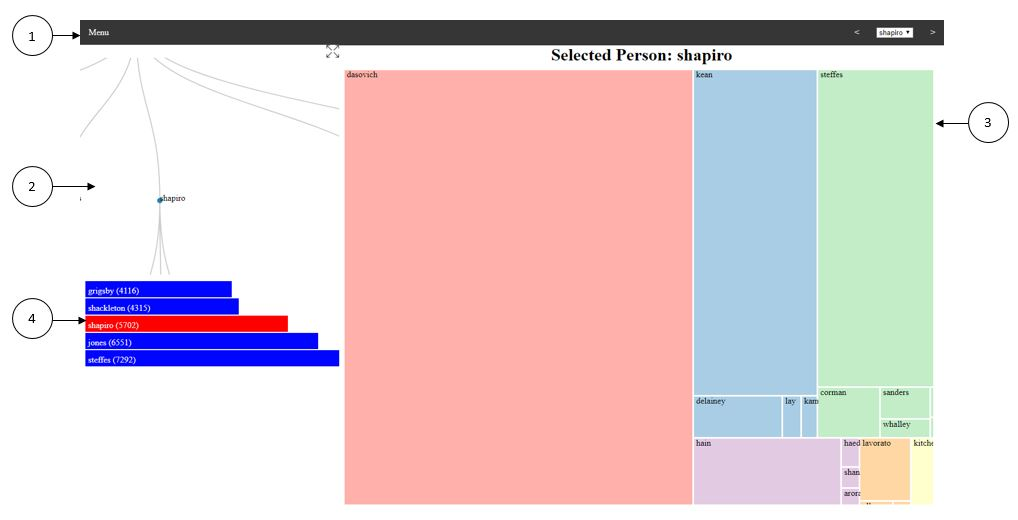
\includegraphics[width=\columnwidth]{pics/whole_app_numbers.jpg}
  \caption[All panels]{Four panels: 1. Menu; 2. Global navigation; 3. Information flow; 4. Supply}
  \label{fig:allpanels}
\end{figure}

\subsubsection{Menu panel}

The \emph{menu panel} is a generic menu, and allows the user to do configure the application such as specifying the data set, exporting results, and providing context about which perspective the user is viewing the data from. This section is supplemental to the visualization. The menu bar will include forward and backward buttons to enable quick and reversible exploration of the data.

\subsubsection{Global navigation panel}

\begin{figure}
  \centering
  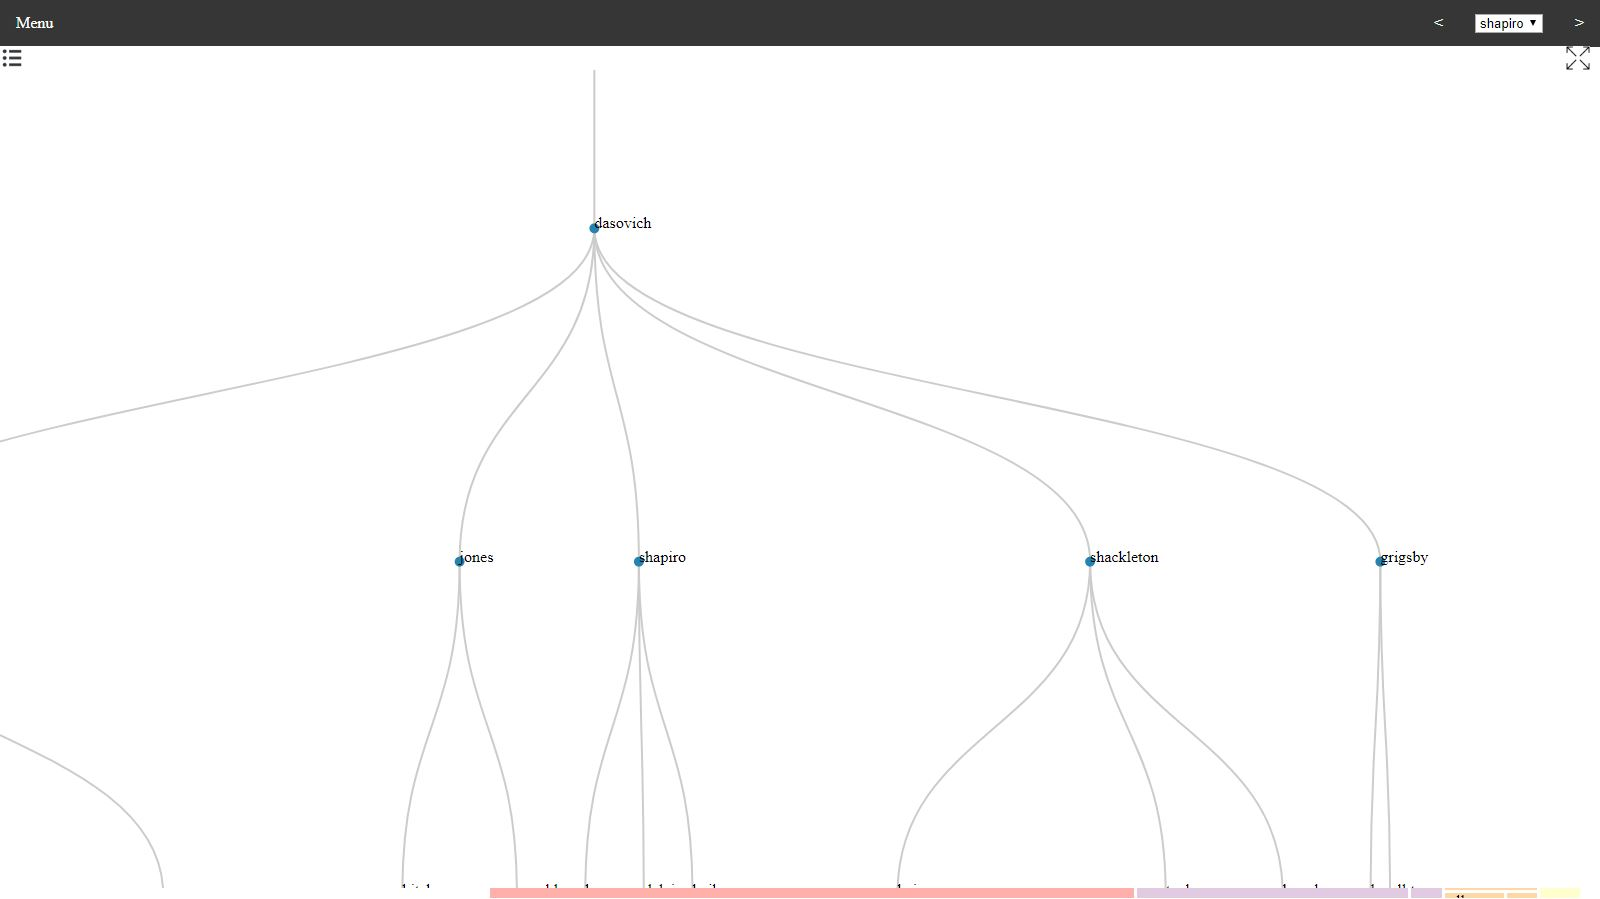
\includegraphics[width=\columnwidth]{pics/expanded_app.jpg}
  \caption{Global navigation panel, expanded}
  \label{fig:global}
\end{figure}


The \emph{global navigation panel} presents a tree graph linking people together in an organizational hierarchy. When the user selects a node in the global navigation panel it will reorient the information flow and supply panel to the egocentric perspective of the person node selected on the global navigation view. This panel allows users to “drill down and find more data about anything that seems important”\cite{ware2012information}.

Organizational structures are typically quite large, so we must afford the ability to keep the size of the visualization manageable---a classic problem in tree graphs\cite{herman2000graph}.  To aid the user with this problem, users will be able to pan and zoom the organizational chart to hone in on areas of particular interest. Figure \ref{fig:global} shows We will also cluster data together, and nodes in the tree will be collapsible and expandable. The panel will also be expandable and collapsible on demand.

Further support for the problems associated with displaying large amounts of data will be provided in the form of filter criteria.  Our visualization will allow the user to filter based on two criteria: number of emails and name. The results of the filter will be applied instantly, where nodes not matching the filtering criteria will be de-emphasized by a reduction in opacity. We chose to de-emphasize nodes instead of removing them entirely to preserve context. Consistent with Shneiderman's rules for filters, our filters will be rapid, incremental and reversible changes to query patterns\cite{ahlberg1994visual}.

When a user hovers over a node in the organization chart it will display links between people in the organization who have formed relationships through email. The relationship uncovered by analysis of email communication is of a different type than the relationship expressed in an org-chart. Colour is “excellent for labeling and categorization”\cite{ware2012information}, so we communicate to the user that the two relationships are different by colouring the links differently in each case.

We use the colour to saliently cue\cite{ware2012information} information in the global navigation panel in at least two other ways: by colouring the selected node differently from the non-selected nodes, and by using colour to trace the user's path through the nodes in the global navigation panel. 

\subsubsection{Information flow panel}

The \emph{information flow panel} contains a treemap of individuals with whom the selected person has a relationship. We chose a tree map to depict the relationships between employees for two reasons. First, its proportional nature allows the visualization to scale from a very small organization, to a very large organization where a person could interact with 100+ people on a regular basis. Second, it communicates the strength of relationship in a salient manner through the size of the rectangles.

We will use colour to group together individuals from the same department to help users easily understand which departments would be most affected if that person was no longer with the organization.  Additional details on demand\cite{anafigueiras} such as email address and department name will be provided through tool tips.  will provide additional details on demand. 

\subsubsection{Supply panel}

After the user has refined the visualization to the person they are interested in and explored / understands how information flows between the person and the rest of the organization, they can begin the managerial decision-making process. The \emph{supply panel} presents all the users in the selected user's group. We present the people in the selected user's group because replacements for a given employee will typically come from the same department of that employee. Each user is presented as a bar in a bar chart, where the height of the bar is determined by the total number of emails sent by that user (which is an indication of their relative workload). Again, we use colour to denote the selected person.  By clicking on the bar chart, the user navigates to that user, and the other panels update accordingly.

The goal of our visualization is best described by Yi, Kang, Stasko, and Jacko: “harnessing human’s remarkable visual perception capabilities to help identify trends, patterns, and unusual occurrences in datasets”\cite{yi2007toward}.  In our specific context this is supporting the user’s decision-making process about organizational change.  We are confident our design meets this objective by using all the relevant elements discussed in class.

\subsection{Development Technology}
Our visualization could be implemented using any number of technologies, however we have chosen a JavaScript based stack.  This choice allows the visualization to be cross platform and take advantage of client-side computer resources such as a GPU.  A server will be required to transform the stored data into a form that is digestible by front end libraries.

Our final visualization will require the use of MySQL, PHP, D3, Perl, and Python.

Pre-processing of project data is required prior to ingest and storage in a database.  The Carnegie Mellon Enron email dataset\cite{cmuenron} contains the email boxes of 148 users.  This real-world data set will be the basis for our project to demonstrate the power of our visualization.  During the pre-processing phase Python and Perl are required for parsing the raw email format and extracting the SMTP header information we require for our project.  The SMTP header information will be augmented with additional attributes that are required to illustrate the various features of our visualization.  The processed data will be stored in a MySQL database.  A database was required due to the volume of data and a requirement to access the data in subsets based on user interaction with the visualization.  Additional data preprocessing will be limited since the class is focused on visualization of data and not data modeling.  The value model chosen will be limited to number of emails sent and not a more elaborate model requiring additional data sets and data manipulation.   

PHP will be used to transform the data model stored in the MySQL database to JSON, which is the primary input format used by D3.  PHP will be further leveraged to do any server-side dynamic web development.

We conducted a thorough review of JavaScript visualization frameworks.  Our research concluded that D3 was the most widely used and mature framework.  After reviewing D3 it met many criteria that we were searching for in a visualization framework.  This included a mature framework that would allow us to focus on implementing our visualization without fear of running into bugs or incomplete code.  It provides the ability to customize every detail of a visualization and its interaction or use high level abstractions that produce generic visualizations out of the box.  Lastly, it provided all the visualizations we required in one library.  We require hierarchical tree view, tree maps, and bar charts.  D3 visualizations come default with a number of features such as zoom and pan, and built in methods to access click functions.  Together this package represents a rapid way to implement our visualization in a robust package that has been tested to work across many platforms.

Eric has a moderate understanding of D3 and increasing his knowledge of MySQL and PHP.  Rob has extensive experience with MySQL, Perl, Python, PHP and increasing his knowledge of D3 rapidly.

\subsection{Project Plan}
\begin{description}[leftmargin=7em, style=nextline]
\item [26 Oct 2018] Submission of Project Proposal
\item [04 Nov 2018] Complete Preliminary Visualization
\item [11 Nov 2018] Complete Review of Visualization
\item [18 Nov 2018] Complete Refinements Based on Visualization Review
\item [25 Nov 2018] Complete 2nd Review of Visualization
\item [30 Nov 2018] Complete Refinements and Presentation
\item [14 Dec 2018] Submit Final Paper
\end{description}


\printbibliography

\end{document}
